\documentclass[
    25pt,
    a0paper,
    portrait,
    colspace=2cm,
    blockverticalspace=2cm
]{tikzposter}

% \usepackage{lmodern}
\usepackage{amsmath}
\usepackage{amssymb}
\usepackage{physics}
\usepackage{bm}
\usepackage{blindtext}

\usetikzlibrary{patterns}

% Turn off the tikzposter watermark
% \tikzposterlatexaffectionproofoff

%% THEMING
%%--------------------------------------------------
%% THEMING
%%--------------------------------------------------

%%--------------------------------------------------
%% FONTS
%%--------------------------------------------------
\usepackage{fontspec}
\usepackage{anyfontsize}
\usepackage[sfdefault]{FiraSans}
\usepackage[scaled=1.15]{newtxmath}

%&--------------------------------------------------
%& COLORS
%%--------------------------------------------------

%%% IBM Carbon colorscheme
%%% https://carbondesignsystem.com/guidelines/color/overview/
\definecolor{Foreground}{RGB}{22, 22, 22}
\definecolor{Background}{RGB}{244, 244, 244}
\definecolor{Blue100}{RGB}{0, 17, 65}
\definecolor{Blue90}{RGB}{0, 29, 108}
\definecolor{Blue80}{RGB}{0, 45, 156}
\definecolor{Blue70}{RGB}{0, 67, 206}
\definecolor{Blue60}{RGB}{15, 95, 254}
\definecolor{Blue50}{RGB}{69, 137, 255}
\definecolor{Blue40}{RGB}{120, 169, 255}
\definecolor{Blue30}{RGB}{166, 200, 255}
\definecolor{Blue20}{RGB}{208, 226, 255}
\definecolor{Blue10}{RGB}{237, 245, 255}
\definecolor{Red}{RGB}{218, 30, 40}
\definecolor{Orange}{RGB}{255, 131, 43}
\definecolor{Yellow}{RGB}{253, 220, 105}
\definecolor{Green}{RGB}{25, 128, 56}
\definecolor{Grey05}{RGB}{240, 240, 240}
\definecolor{Grey10}{RGB}{224, 224, 224}
\definecolor{Grey15}{RGB}{211, 211, 211}
\definecolor{Grey20}{RGB}{198, 198, 198}
\definecolor{Grey30}{RGB}{168, 168, 168}
\definecolor{Grey40}{RGB}{141, 141, 141}
\definecolor{Grey50}{RGB}{111, 111, 111}
\definecolor{Grey60}{RGB}{82, 82, 82}
\definecolor{Grey70}{RGB}{57, 57, 57}
\definecolor{Grey80}{RGB}{38, 38, 38}
\definecolor{Grey90}{RGB}{22, 22, 22}
\definecolor{White}{RGB}{255, 255, 255}
\definecolor{Black}{RGB}{0, 0, 0}

\definecolorstyle{MyColorStyle}{
    % Random colors
    \definecolor{colorOne}{named}{Blue70}
    \definecolor{colorTwo}{named}{Green}
    \definecolor{colorThree}{named}{Red}
}{
    % Background Colors
    \colorlet{backgroundcolor}{White}
    \colorlet{framecolor}{Grey50}
    % Title Colors
    \colorlet{titlefgcolor}{Background}
    \colorlet{titlebgcolor}{colorOne}
    % Block Colors
    \colorlet{blocktitlebgcolor}{Background}
    \colorlet{blocktitlefgcolor}{colorOne}
    \colorlet{blockbodybgcolor}{Background}
    \colorlet{blockbodyfgcolor}{Foreground}
    % Innerblock Colors
    \colorlet{innerblocktitlebgcolor}{Grey10}
    \colorlet{innerblocktitlefgcolor}{colorTwo}
    \colorlet{innerblockbodybgcolor}{Grey10}
    \colorlet{innerblockbodyfgcolor}{Foreground}
    % Note colors
    \colorlet{notefgcolor}{black}
    \colorlet{notebgcolor}{colorTwo!50!white}
    \colorlet{noteframecolor}{colorTwo}
}

\usecolorstyle{MyColorStyle}


%%--------------------------------------------------
%% BACKGROUND
%%--------------------------------------------------
\definebackgroundstyle{MyBackground}{
    \fill[
        backgroundcolor,
        inner sep=0pt,
        line width=0pt,
    ] (bottomleft) rectangle (topright);
}

\usebackgroundstyle{MyBackground}


%%--------------------------------------------------
%% BLOCKS
%%--------------------------------------------------
\defineblockstyle{MyBlockStyle}{
    titlewidthscale=1,
    bodywidthscale=1,
    titlecenter,
    titleoffsetx=0pt,
    titleoffsety=10pt,
    bodyoffsetx=0mm,
    bodyoffsety=15mm,
    bodyverticalshift=5mm,
    roundedcorners=0,
    linewidth=1pt,
    titleinnersep=1.2cm,
    bodyinnersep=1.2cm
}{
    \ifBlockHasTitle
        % Body
        \fill[
            blockbodybgcolor,
            rounded corners=\blockroundedcorners,
            line width=\blocklinewidth
        ] (blockbody.south west) rectangle (blockbody.north east);
        % Block Title
        \fill[
            fill=blockbodybgcolor,
            rounded corners=\blockroundedcorners,
            line width=\blocklinewidth
        ] (blocktitle.south west) rectangle (blocktitle.north east);
    \else
        % Only body
        \fill[
            blockbodybgcolor,
            rounded corners=\blockroundedcorners,
            line width=2\blocklinewidth
        ] (blockbody.south west) rectangle (blockbody.north east);
    \fi
}

\defineinnerblockstyle{MyInnerBlockStyle}{
    titlewidthscale=1,
    bodywidthscale=1,
    titleleft,
    titleoffsetx=0pt,
    titleoffsety=0pt,
    bodyoffsetx=0mm,
    bodyoffsety=0mm,
    bodyverticalshift=-10mm,
    roundedcorners=0,
    linewidth=1pt,
    titleinnersep=0.8cm,
    bodyinnersep=0.8cm
}{
    % Body
    \fill[
        innerblockbodybgcolor,
        rounded corners=0,
        line width=\innerblocklinewidth
    ] (innerblockbody.south west) rectangle (innerblockbody.north east);
    % Block Title
    \fill[
        innerblocktitlebgcolor,
        rounded corners=0,
        line width=\innerblocklinewidth
    ] (innerblocktitle.south west) rectangle (innerblocktitle.north east);
}

\useblockstyle{MyBlockStyle}
\useinnerblockstyle{MyInnerBlockStyle}
\newcommand{\myblock}[2]{\block{{\LARGE \bfseries \sffamily \addfontfeature{LetterSpace=3.0} #1}}{\large #2}}


%%--------------------------------------------------
%% TITLE
%%--------------------------------------------------
\definetitlestyle{MyTitle}{
    width=\textwidth,
    roundedcorners=0,
    linewidth=4pt,
    innersep=1.5cm,
    titletotopverticalspace=-1mm,
    titletoblockverticalspace=15mm
}{
    \begin{scope}[line width=\titlelinewidth]
        \fill[
            fill=Foreground
        ] (\titleposleft, \titleposbottom) rectangle (\titleposright, \titlepostop);
        \draw[color=titlebgcolor, line width=10, shorten <=-3pt, shorten >=-3pt]
            (\titleposleft, \titleposbottom) -- (\titleposright, \titleposbottom);
        \path (\titleposleft, \titlepostop) -- ++(0, -1) node [anchor=north west, inner sep=20pt] {
\includegraphics[scale=1.2]{figures/unibo_neg.pdf}};
        \path (\titleposright, \titlepostop) -- ++(-0.5, -2) node [anchor=north east, inner sep=20pt] {
\includegraphics[scale=0.6]{figures/infn_logo_neg.pdf}};
    \end{scope}
}
\usetitlestyle{MyTitle}

\settitle{
    \centering
    \vbox{
        \vspace*{0.25cm}
        \centering \color{titlefgcolor} {\sffamily \bfseries \Huge \addfontfeature{LetterSpace=5.0} \@title \par}
        \vspace*{0.5cm}
        {\sffamily \Large \@author}\\
        \vspace*{0.25cm}
        {\sffamily {\slshape \@institute}}
    }
}

% vim: nospell

\newcommand{\Note}[1]{
    \vspace*{0.5cm}
    \hfill \textit{#1}
}

%% TITLE
%%--------------------------------------------------
\title{QUANTUM FISHER INFORMATION AND TOPOLOGICAL PHASES}
% FIXME:
%   Non è il titolo dell'abstract mandato.
%   Il titolo originale: "Quantum Fisher information as a tool for detecting topological spaces"
%   non ci sta nel riquadro
\author{Sunny Pradhan, Federico dell'Anna, Elisa Ercolessi}
\institute{University of Bologna}




\begin{document}

\maketitle

\block[bodyverticalshift=5mm]{}{\Large
We study the Quantum Fisher Information (QFI) in one-dimensional models as a tool for measuring the Multipartite Entanglement (ME), which can give valuable information about the existence of topological phases.
We show that the scaling of the QFI of strictly non-local observables can be used for characterizing the phase diagrams and, in particular, for detecting topological phases, where it scales maximally.
}


\begin{columns}
    \column{0.5}
    \myblock{MULTIPARTITE ENTANGLEMENT}{
        \innerblock{$n$--separability}{
            \begin{equation*}
                \ket{\psi} = \ket{\phi_1} \otimes \ket{\phi_2} \otimes \cdots \otimes \ket{\phi_n}
            \end{equation*}

            \Note{factorizable in $n$ terms}
        }
        \vspace*{1cm}
        \innerblock{$k$--producibility}{
            \begin{equation*}
                \ket{\psi} = \ket{\phi_1} \otimes \ket{\phi_2} \otimes \cdots \otimes \ket{\phi_m}
            \end{equation*}

            \Note{each term involves at most $k$ elements}
        }
    }
    \myblock{QUANTUM FISHER INFORMATION}{
        Unitary transformation with \textbf{unknown angle} $\theta$
        $$\rho \to \rho(\theta) = e^{-i \theta \hat{H}} \rho e^{i \theta \hat{H}}$$

        Angle $\theta$ to be estimated with $m$ measurements and operators $\{\hat{E}_{\mu}\}$

        \vspace*{1cm}

        \innerblock{Fisher information}{
            \begin{equation*}
                F[\rho(\theta), \{\hat{E}_{\mu}\}] = \sum_{\mu} \frac{ [\partial_{\theta} P(\mu|\theta)]^2}{P(\mu | \theta)}
                \qquad
                P(\mu | \theta) = \Tr[\rho(\theta) \hat{E}_{\mu}]
            \end{equation*}

            \Note{$P(\mu | \theta)$ conditional probabilities of a measure $\mu$ given $\theta$}
        }

        \vspace*{1cm}

        \innerblock{Quantum Fisher information}{
            \begin{equation*}
                F_Q[\rho, \hat{H}] = \max_{\{\hat{E}_{\mu}\}} F[\rho(\theta), \{\hat{E}_{\mu}\}]
            \end{equation*}

            \Note{maximum of $F$ over the set of possible measures $\{\hat{E}_{\mu}\}$}
        }
    }

    \column{0.5}
    \myblock{LONG-RANGE KITAEV CHAIN}{
        \innerblock{one-dimensional $p$-wave superconductor}{
        \begin{equation*}
            H = \sum_{i} \qty[
                -t c_i^{\dagger} c_j
                -\mu \qty( c_j^{\dagger} c_j - \frac{1}{2} )
                + \frac{\Delta}{2} \sum_{r} \frac{1}{r^{\alpha}} c_j^{\dagger} c_{j+r}
                + \text{h.c.}
            ]
        \end{equation*}

        \Note{long-range coupling $\sim 1/r^{\alpha}$}
        }

        \begin{tikzfigure}
            \begin{tikzpicture}[
    scale=2.5,
    font=\normalsize,
    punto/.style = {circle, inner sep=0pt, minimum size=5pt, fill=black},
    massless/.style = {fill=Green, fill opacity=0.8},
    trivial/.style = {fill=Blue20, fill opacity=0.8},
    massive/.style = {fill=Orange, fill opacity=0.8},
    etichetta/.style = {fill=white, fill opacity=0.9, text opacity=1, rounded corners, inner sep=5pt},
    etichetta spettro/.style = {above=-0.25cm, font=\small, fill=Grey10, fill opacity=0.9, text opacity=1, rounded corners, inner sep=5pt}
    ]

    %%% Phases
    % massless
    \path[massless] (-2,1) rectangle (2,3);
    % massive
    \path[massive]  (-4,1) rectangle (2,0);
    % trivial
    \path[trivial] (-4,1) rectangle (-2,3);
    \path[trivial] (2,0) rectangle (4,3);


    % sector separator
    \draw[dashed, line width=3pt] (-4.2,1) -- (4.4,1) node [pos=0.95, below, etichetta] {$\alpha = 1$};

    % critical line
    \draw[line width=7] (2,0) -- (2,3);
    \draw[dotted]     (-2,0) -- (-2,1);
    \draw[line width=7] (-2,1) -- (-2,3);

    %%% Axis
    \draw[ultra thick, ->] (0,0) -- (0,3.2) node [above] {$\alpha$};
    \draw[ultra thick, ->] (-4.2,0) -- (4.2,0) node [right] {$\mu$};
    \draw (2,0) node [below] {$2$};
    \draw (-2,0) node [below] {$-2$};
    \draw (0,0) node [below] {$0$};


    % labels
    \node [etichetta] (massless) at (0,2)  {topol.~massless};
    \node [etichetta] (trivial1) at (-3,2.25) {trivial};
    \node [etichetta] (trivial2) at (3,2.25)  {trivial};
    \node [etichetta] (massive)  at (-1,0.5)  {topol.~massive};

    \draw[<-, ultra thick] (2,3.1) -- (2,3.3) node [above] {critical};
    \draw[<-, ultra thick] (-2,3.1) -- (-2,3.3) node [above] {critical};

    \draw (-4, 2)    node [anchor=south, etichetta, rotate=90] {\textbf{Majorana}};
    \draw (-4, 0.5)  node [anchor=south, etichetta, rotate=90] {\textbf{Dirac}};

    % energy plots
    \node[anchor=west] (MajSpec) at (5, 2) {\FrameImg{0.8}{figures/majorana_spectrum.pdf}};
    \node[etichetta spettro] at (MajSpec.north) {Majorana sector, $\alpha = 2$};
    \node[anchor=west] (DiracSpec) at (5, -1.3) {\FrameImg{0.8}{figures/dirac_spectrum.pdf}};
    \node[etichetta spettro] at (DiracSpec.north) {Dirac sector, $\alpha = 0.7$};

    \draw[ultra thick] (massless.south east) edge[->, bend right=20] (MajSpec.west);
    \draw[ultra thick] (massive.south east)  edge[->, bend right=20] (DiracSpec.west);

    % Annotate Majorana plot
    \begin{scope}[xshift=5cm, yshift=2cm]
        \node (MasslessEdge) [etichetta, font=\tiny, anchor=south] at (2.5, -0.30) {\textbf{massless} edge state};
        \draw[ultra thick, ->] (MasslessEdge.south) -- ++(0,-0.3);
        \node[font=\tiny] at (2.5, 0.95) {\textbf{topological}};
        \node[font=\tiny] at (1.0, 0.95) {trivial};
        \node[font=\tiny] at (4.0, 0.95) {trivial};
    \end{scope}

    % Annotate Dirac plot
    \begin{scope}[xshift=5cm, yshift=-1.3cm]
        \node (MassiveEdge) [etichetta, font=\tiny, anchor=south] at (2.5, 0.2) {\textbf{massive} edge state};
        \draw[ultra thick, ->] (MassiveEdge.south west) -- ++(-0.17, -0.17);
        \node[font=\tiny] at (2.4, 0.95) {\textbf{topological}};
        \node[font=\tiny] at (4.0, 0.95) {trivial};
    \end{scope}
\end{tikzpicture}

        \end{tikzfigure}
    }

    \myblock{BILINEAR--BIQUADRATIC CHAIN}{
        \innerblock{Spin-1 chain}{
            \begin{equation*}
                H = J \sum_{i} \qty[
                    \bm{S}_i \cdot \bm{S}_{i+1}
                    + \beta \qty( \bm{S}_i \cdot \bm{S}_{i+1} )
                ]
            \end{equation*}
        }

        \begin{tikzfigure}
            \begin{tikzpicture}[
        scale=5,
        font=\normalsize,
        dot/.style = {circle, inner sep=0pt, minimum size=10pt, fill=black},
        line width=2pt,
        etichetta grafico/.style = {above=0.1cm, font=\normalsize, fill=Grey10, fill opacity=0.9, text opacity=1, rounded corners, inner sep=5pt},
        nota grafico/.style = {below=0.2cm, font=\small, fill=Grey10, fill opacity=0.9, text opacity=1, rounded corners, inner sep=5pt, align=center},
        sfondo grafico/.style = {fill=white, draw=black, thin, inner sep=5pt}
    ]
    \node (A) at (45:1)  [dot] {};
    \node (C) at (-45:1) [dot] {};
    \node (D) at (-90:1) [dot] {};
    \node (E) at (135:1) [dot] {};
    \node (H) at (0:1)   [dot] {};
    \node (K) at (-18.44:1) [dot] {};
    \node[above right] at (A) {$\pi/4$};
    \node[below right] at (C) {$-\pi/4$};
    \node[below]       at (D) {$-\pi/2$};
    \node[above left]  at (E) {$3 \pi / 4$};
    \node[right]       at (H) {Heisenberg};
    \node[right]       at (K) {\textbf{AKLT}};

    \draw (0,0) circle [radius=1];

    \draw[fill=Blue40, fill opacity=0.7] (0,0) -- (C) arc (-45:45:1) -- (0,0);
    \draw[fill=Green, fill opacity=0.5] (0,0) -- (D) arc (-90:-45:1) -- (0,0);
    \draw[fill=Red, fill opacity=0.5] (0,0) -- (A) arc (45:135:1) -- (0,0);

    \node at (45:1)  [dot] {};
    \node at (-45:1) [dot] {};
    \node at (-90:1) [dot] {};
    \node at (135:1) [dot] {};
    \node at (0:1)   [dot] {};
    \node at (-18.44:1) [dot] {};

    \path (A) arc (45:135:1) node [below=10pt, midway] {Dimer};
    \path (C) arc (-45:45:1) node [left=6pt, midway] {Haldane};
    \path (D) arc (-90:-225:1) node [above right=10pt, midway] {Ferro};
    \path (C) arc (-45:-90:1) node [above=8pt, pos=0.6] {Trimer};

    \draw[freccia] (10:1.1) arc (10:35:1.1) node [midway, right] {$\theta = \tan^{-1} \beta$};

    % Disegni diagrammi di fase
    \node (AKLTstate) [anchor=west] at (2.5, 0.2) {\begin{tikzpicture}[
        spin one/.style={fill=Blue20, fill opacity=1, draw=black, thin, inner sep=0pt, minimum size=5pt, thick},
        spin half/.style={circle, fill=Orange, draw=black, inner sep=0pt, minimum size=0.5cm},
        entangled/.style={line width=4pt},
        nonentangled/.style={dotted, thick},
        font=\footnotesize
        ]
        % spin 1 sites
        \foreach \x in {0, 3, ..., 15}
            \draw [spin one] (\x, 0) ellipse [ x radius=1cm, y radius=0.5cm ];

        % entanglement lines
        \foreach \x/\y in {0/3, 3/6, 6/9, 9/12, 12/15}
            \draw[entangled] (\x+0.4,0 ) -- (\y-0.4,0);
        \draw[entangled] (-1.5, 0) -- (-0.4, 0);
        \draw[entangled] (15.4, 0) -- (16.5, 0);

        % spin one half lines
        \foreach \x in {0, 3, ..., 15} {
            \draw (\x+0.1, 0) node [spin half] {};
            \draw (\x-0.6, 0) node [spin half] {};
        }

        % labels
        \draw[<-, shorten <=2pt, thick] (3, 0.5) -- +(0, 1) node [above] {spin--$1$};
        \draw[<-, shorten <=1pt, thick] (6.5, 0.2) -- +(1, 1) node  [above right] {spin--$\frac{1}{2}$};
        \draw[<-, shorten <=2pt, thick] (4.5, 0) -- +(0, -1) node [below, align=center] {entangled\\ single pair};

\end{tikzpicture}
 };
    \node [etichetta grafico, above=-1.25cm] at (AKLTstate.north east) {AKLT state $\qty(\beta = -\frac{1}{3})$};
    \node (DimerState) [anchor=west] at (2.5, -0.8) {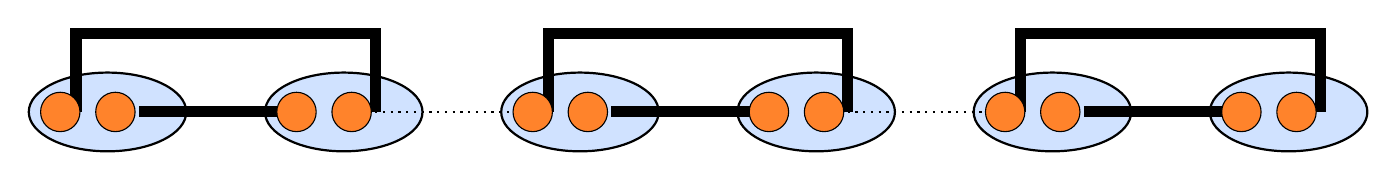
\begin{tikzpicture}[
    spin one/.style={fill=Blue20, fill opacity=1, draw=black, thin, inner sep=0pt, minimum size=5pt, thick},
    spin half/.style={circle, fill=Orange, draw=black, inner sep=0pt, minimum size=0.5cm},
    entangled/.style={line width=4pt},
    nonentangled/.style={dotted, thick},
    font=\footnotesize
    ]
    % spin 1 sites
    \foreach \x in {0, 3, ..., 15}
    \draw [spin one] (\x, 0) ellipse [ x radius=1cm, y radius=0.5cm ];

    % entanglement lines
    \foreach \x/\y in {0/3, 6/9, 12/15} {
        \draw[entangled] (\x+0.4, 0 ) -- (\y-0.4,0);
        \draw[entangled] (\x-0.4, 0 ) -- ++(0, 1) -- ++(3.8, 0) -- ++(0, -1);
    }
    \draw[nonentangled] (3.4, 0) -- (5.6,0);
    \draw[nonentangled] (9.4, 0) -- (11.6,0);

    % spin one half
    \foreach \x in {0, 3, ..., 15} {
        \draw (\x+0.1, 0) node [spin half] {};
        \draw (\x-0.6, 0) node [spin half] {};
    }
\end{tikzpicture}
 };
    \node [etichetta grafico] at (DimerState.north east) {Dimer state};

    % Grafico QFI vs beta
    \node[anchor=north, sfondo grafico] at (0, -1.75) (VarBeta)
        {\begin{tikzpicture}[scale=1.5, font=\tiny]
    \begin{axis}[
        height=7cm,
        width=8cm,
        xlabel=$\beta$,
        ylabel={QFI density},
        ymin=0,
        ymax=17,
        x label style={at={(axis description cs:0.5,-0.1)}, anchor=north},
        y label style={at={(axis description cs:-0.08,.5)}, anchor=south},
        important mark/.style={mark=diamond*, mark options={scale=2, draw=black, thin}}
        ]
        % riquadri colorati
        \fill[Green,  fill opacity=0.5] (axis cs:-3,0) rectangle (axis cs:-1,17);
        \fill[Blue40, fill opacity=0.7] (axis cs:-1,0) rectangle (axis cs:1,17);
        \fill[Red,    fill opacity=0.5] (axis cs: 1,0) rectangle (axis cs:3,17);
        \draw[thin, opacity=0.5, Grey80, thick] (axis cs:-1,0) -- (axis cs:-1,17);
        \draw[thin, opacity=0.5, Grey80, thick] (axis cs:1,0) -- (axis cs:1,17);

        % dati
        \addplot[black, mark=*, only marks] table {figures/data/fisher_beta.dat};
        \addplot[Red,  important mark] coordinates { (1,3.812) };
        \addplot[Blue70, important mark] coordinates { (-0.333333, 13.5556) };

        % phases
        \node [] at (axis cs: 0, 16.7) {Haldane};
        \node [] at (axis cs: -1.6, 16.7) {Trimer};
        \node [] at (axis cs: 1.6, 16.7) {Dimer};

        % notes
        \node[anchor=center] (AKLT) at (axis cs:-0.333333, 13.5556) {};
        \node[anchor=center] (critical) at (axis cs:1, 3.812) {};
        \draw[Stealth-, thick] (AKLT.west) -- (axis cs: -1.2, 12) node [anchor=east, etichetta] {AKLT};
        \draw[Stealth-, thick] (critical.north) -- (axis cs: 1.2, 8) node [anchor=south, etichetta] {critical};
    \end{axis}
\end{tikzpicture}
};
    \node[etichetta grafico] at (VarBeta.north) {\textbf{QFI density ~vs~ $\bm{\beta}$}};
    \node[nota grafico] at (VarBeta.south) {$f_Q$ grows inside the Haldane phase \\and is maximum on the AKLT point};


    % Grafici QFI nella fase Haldane e beta=1
    \node[right=2cm of VarBeta.north east, anchor=north west, sfondo grafico]
        (Haldane) {\begin{tikzpicture}[
        scale=1.5,
        font=\tiny,
        important mark/.style={mark=diamond*, only marks, mark options={scale=2, draw=black, thin}},
        normal mark/.style={mark=*, only marks, mark options={draw=black, thin}}
    ]
    % \clip (-1.3, -1.3) rectangle (6.4, 5.7);
    \begin{axis}[
        height=7cm,
        width=8cm,
        xmin=0,
        ymin=0,
        ymax=15,
        xlabel={chain size},
        ylabel={QFI density},
        x label style={at={(axis description cs:0.5,-0.1)}, anchor=north},
        y label style={at={(axis description cs:-0.08,.5)}, anchor=south},
        fit/.style={gray, very thick, domain=4:33, no marks}
        ]
        \addplot[Blue70,  important mark] table {figures/data/beta=-0.333.dat};
        \addplot[red,   normal mark] table {figures/data/beta=0.dat};
        \addplot[green, normal mark] table {figures/data/beta=0.333.dat};
        \addplot[cyan,  normal mark] table {figures/data/beta=0.666.dat};

        % fit ottenuti con numpy.polyfit
        \addplot[fit] {0.4440*x + 0.2300 } node [pos=0.7, above, sloped, etichetta] {$\beta=-1/3$}; % beta = -1/3
        \addplot[fit] {0.3556*x + 0.3449 } node [pos=0.8, below, sloped, etichetta] {$\beta=0$}; % beta = 0
        \addplot[fit] {0.1970*x + 1.1224 } node [pos=0.95, below, sloped, etichetta] {$\beta=1/3$}; % beta = 1/3
        \addplot[fit] {0.1117*x + 1.5504 } node [pos=0.9, below, sloped, etichetta] {$\beta=2/3$}; % beta = 2/3

        \node[etichetta] at (axis description cs: 0.1, 0.8)  {$f_Q \sim L$};
    \end{axis}
\end{tikzpicture}
 };
    \node[etichetta grafico] at (Haldane.north) {Inside \textbf{Haldane phase}};
    \node[nota grafico] at (Haldane.south) {$f_Q$ scales \emph{linearly} inside \\the Haldane \emph{topological} phase};

    % Grafici QFI nella fase Haldane e beta=1
    \node[right=2cm of Haldane.north east, anchor=north west, sfondo grafico]
        (Beta1) {\begin{tikzpicture}[
        scale=1.5,
        font=\tiny,
        ]
    \begin{axis}[
        height=5cm,
        width=8cm,
        xmin=0,
        ymin=0,
        xlabel={chain size},
        ylabel={QFI density},
        x label style={at={(axis description cs:0.5,-0.12)}, anchor=north},
        y label style={at={(axis description cs:-0.08,.5)}, anchor=south},
        fit/.style={gray, very thick, domain=1:33, no marks}
        ]
        \addplot[Red, mark=diamond*, mark options={scale=2, draw=black, thin}] table {figures/data/beta=1.dat};

        % dati fit ottenuti con scipy.optimize.curve_fit
        \addplot[fit] {0.2299 + 0.8046*(x^0.4391)} node [midway, below=8pt, etichetta] {$\beta=1$};

        \node[etichetta] at (axis description cs: 0.6, 0.3)  {$f_Q \sim L^{0.44}$};
    \end{axis}
\end{tikzpicture}
 };
    \node[etichetta grafico] at (Beta1.north) {\textbf{Critical point} $\beta = 1$ ($\theta = \pi/4$)};
    \node[nota grafico] at (Beta1.south) {$f_Q$ scales with a \emph{power-law} for \\a quantum phase transition point};

\end{tikzpicture}


        \end{tikzfigure}
    }

\end{columns}


\end{document}
